\documentclass[10pt, openany]{book}

\usepackage{fancyhdr}
\usepackage{imakeidx}

\usepackage{amsmath}
\usepackage{amsfonts}

\usepackage{geometry}
\geometry{letterpaper}

\usepackage{fancyvrb}
\usepackage{fancybox}

\usepackage{url}
\usepackage{gensymb}
\usepackage{multicol}
\usepackage{tabularx}
%
% Rules to allow import of graphics files in EPS format
%
\usepackage{graphicx}
\DeclareGraphicsExtensions{.eps}
\DeclareGraphicsRule{.eps}{eps}{.eps}{}
%
% Macro definitions
%
\newcommand{\switch}[2]{``#1''/``#2''}
\newcommand{\position}[1]{``#1''}
%
% Front Matter
%
\title{Raspberry Pi Based Mainframe Simulator}
\author{Brent Seidel \\ Phoenix, AZ}
\date{ \today }
%========================================================
%%% BEGIN DOCUMENT
\begin{document}
%
% Produce the front matter
%
\frontmatter
\maketitle
\begin{center}
This document is \copyright 2021 Brent Seidel.  All rights reserved.

\paragraph{}Note that this is a draft version and not the final version for publication.
\end{center}
\tableofcontents
\listoffigures
\listoftables

\mainmatter
%----------------------------------------------------------
\chapter{Introduction}
A rather simplistic view is that this provides a way to get a Raspberry Pi to blink some LEDs and read some switches.  However, this hardware could be modified for a number of other applications that require lots of discrete I/O, such as burglar alarms or sprinkler controls.

\section{Parts}
\subsection{3D Printing}
A fair bit of 3D printing is required, so having lots of filament is a good idea.  Labels on the panels are done by (on my printer with a 0.15mm layer height) printing 2 layers of the panel color, then 3 layers of a contrasting color for the text, and then the rest in the panel color.  The panels are printed with the text faced down.  You may wish to tinker with this for your printer.  The actual parts are:
\begin{itemize}
  \item Four or six racks depending on whether you want a 16 or 32 bit system.
  \item One processor tray.
  \item Two or three discrete I/O trays.
  \item One control panel
  \item One modes panel
  \item Two or four address/data panels (starting at 0, 8, 16, and 24).
\end{itemize}

\subsection{Electronic Parts}
Note that soldering will be required so a soldering station with appropriate tools and solder will be required in addition to the following.
\begin{itemize}
  \item One Raspberry Pi 3B computer (available from many places).
  \item Four or six half-size perma-proto breadboards (p/n 1609 for qty 1 or p/n 571 for qty 3 from Adafruit)\footnote{Adafruit generally throws one of these in with your order if your order is over \$100}.
  \item One quarter-size perma-proto breadboard (p/n 1608 from Adafruit).
  \item At least four or up to eight MCP23017 I2C 16 bit input/output port expander chips (p/n 732 from Adafruit).
  \item One 28-pin DIP socket per MCP23017.  (eg p/n A120353-ND from Digi-Key)
  \item Recommended one LTC4311 I2C Extender/Active Terminator (p/n 4756 from Adafruit).
  \item One set of Female/Male jumper wires (p/n 1954 from Adafruit).  These are used to connect from the Raspberry Pi to the rest of the circuitry since female connectors are needed on the Raspberry Pi end).
  \item Hookup wire, preferably multi-colored (available from many places).
  \item 36 pin 0.1'' female header (5 pack p/n 598 at Adafruit).  You may need a couple packs.
  \item 23 to 39 Mini panel mount SPDT toggle switches (p/n 3221 from Adafruit).  Feel free to use other switches if you like, though you may need to adjust the hole sizes in the panels.
  \item 11 or 16 female and male DB-9 connectors (eg p/n AE10972-ND (male) and p/n AE11063-ND (female) from Digi-Key (buy a pack of 25 for a price discount)).
  \item Lots of 5mm oval LEDs (I used red, but you can use other colors) (eg p/n C5SMF-RJF-CT0W0BB1-ND from Digi-Key (buy a pack of 100 for a price discount, you can always use the excess in other projects)).
  \item Lots of 120$\Omega$ resistors (eg p/n CF14JT120RCT-ND (lots of other options) from Digi-Key).  These are used for current limiting the LEDs from 3.3V drive.  If you're driving the LEDs with 5V, you'll need a bit more resistance.  Since the Raspberry Pi uses 3.3V, these will work for this project.
  \item A couple meters of CAT-5 cable.  This is for the cables to connect the various assemblies (available from many places).
\end{itemize}

\subsection{Mechanical Hardware}
I have a Phillips Panhead Electronic Hardware Kit from Digi-Key (p/n 1602-KIT-ND) that has an assortment of machine screws and nuts.  I used these because they were handy.

You will need many cable ties.  I have a container of assorted cable ties from Costco.  These can be obtained from many other sources.

%----------------------------------------------------------
\chapter{Hardware}

\section{Electronics}
\subsection{Processor}
I had a Raspberry Pi 3 board laying around so I figured that I would use it.  Interestingly, this is a more powerful computer than many of the processors it might be used to simulate.

\subsection{Discrete I/O}
Each of these boards in built on a 1/2 size perma-proto board from Adafruit.  It has one MCP23017 16 bit I/O expander chip with I2C interface in a socket.  Three pins are provided to configure the address, so the system can have up to 8 of these chips or 128 discrete I/O pins.  There is space on the board for 8 current limiting resistors for LED drive.

\section{3D Printed Parts}
\subsection{Racks}
Each rack is a bbs\_rack2(10, 6, 4).  The size is basically constrained by what my 3D printer can do.  Each of these requires about 15 hours to print on my printer.  Two of these can be bolted together side-by-side and fit in a 19 inch rack.  This is the approximate size of the classic computer equipment.  Multiple racks can be bolted together vertically as needed to provide panel space.  Each rack has slots for two vertically oriented trays.

\subsection{Processor Tray}
 The processor tray has mounting holes for the Raspberry Pi processor boad. It also has a 1/4 size perma-proto board from Adafruit (this may get changed to a half sized board) to provide space for miscellaneous wiring.  Also on the tray is a LTC4311 I2C Extender/Active Terminator (p/n 4756 from Adafruit).  This may not strictly be necessary, but since the I2C bus will be running off to several other boards, I thought that it might be a good idea.  There is also a DB-9 connector that carries power and the I2C bus to the other trays.

\subsection{Discrete I/O Tray}
Each of these trays has one or two MCP23017 16 bit I/O expander chips with I2C interface.  These trays would typically be mounted in the slot next to the panel.  The tray has 4 DB-9 connections and can interface with up to  16 LEDs and 16 switches.  One additional DB-9 connection is provided to connect the the power and I2C bus from the processor.

\subsection{Address/Data Panels}
The address/data panels provide 8 switches and LEDs numbered consecutively from right to left.  The starting number is selectable in the model.  Each panel has two cables (one for LEDs and one for switches) that attach to connectors on the discrete I/O boards.  Enough of these need to be provided to account for all the address and data lines in the simulated processor.  A system would typically have two or four of these panels for 16 or 32 bit systems.  Note that there are many cases where the number of address lines does not match the number of data lines.  In these cases panels would need to be provided for whichever number is greater.

\subsection{Control Panel}
At this point, without an actual CPU simulation, this is mostly a way to organize what needs to be in a relatively generic control panel.  The following functions are needed:
\begin{itemize}
  \item Read from a memory location.
  \item Write to a memory location.
  \item Stop/pause processor execution.
  \item Start processor execution at a specified address.
  \item Continue processor execution.
  \item Reset the processor.
\end{itemize}

The following switches are defined on the panel:
\begin{itemize}
  \item \switch{Run}{Pause} - The \position{Run} position allows program execution.  The \position{Pause} position temporarily suspends execution.  Moving the switch back to the \position{Run} position will continue where the program left off.
  \item \switch{Start}{Stop} - Moving the switch to the \position{Start} position loads a starting address to begin program execution.  The \position{Stop} position halts a program and a new starting address will need to be provided.
  \item \switch{Auto}{Man} - The \position{Auto} position allows for remote control of the simulator via a web interface.  The \position{Man} position disables remote control.
  \item \switch{Addr}{Data} - Selects display and entry of memory addresses or data.
  \item \position{Dep} deposits the switch value.  If the \switch{Addr}{Data} switch is in the \position{Addr} position, a memory address is loaded.  If the \switch{Addr}{Data} switch is in the \position{Data} position, the switch value is deposited in memory and the address incremented.
  \item \position{Exam} is used to examine memory at the current address.  The address is incremented each time the switch is moved to the \position{Exam} position.
  \item Spare - an empty position reserved for future expansion.
  \item \switch{Power}{Off} - This will eventually be wired up to control power to the Raspberry Pi computer.
\end{itemize}

\subsubsection{To Specify an Address}
Note that if the word size is greater than 8 bits, some of the lower order address bits may be ignored.
\begin{itemize}
  \item Toggle the desired address using the address/data switches.
  \item Move the \switch{Addr}{Data} switch to the \position{Addr} position.
  \item Move the ``Dep'' (deposit) switch to the \position{Dep} position.
  \item Once the LED for the ``Dep'' switch illuminates, move the switch to the unlabeled position.
\end{itemize}

\subsubsection{To Read Memory}
\begin{itemize}
  \item Specify the starting address as described above.
  \item Move the \switch{Addr}{Data} switch to the \position{Data} position.
  \item Move the ``Exam'' switch to the \position{Exam} position.
  \item The contents of memory at the specified address will be displayed in the Address/Data LEDs.
  \item The \switch{Addr}{Data}  switch can be used to toggle between display of the address and the data.
  \item Move the ``Exam'' switch to the unlabeled position.  This increments the internal address pointer so that by toggling this switch a block of memory can be modified.
\end{itemize}

\subsubsection{To Write Memory}
\begin{itemize}
  \item Specify the starting address as described above.
  \item Move the \switch{Addr}{Data}  switch to the \position{Data} position.
  \item Toggle the desired data using the address/data switches.
  \item Move the ``Dep'' switch to the \position{Dep} position.
  \item The contents of memory at the specified address will be updated and displayed in the Address/Data LEDs.
  \item The \switch{Addr}{Data} switch can be used to toggle between display of the address and the data.
  \item Move the ``Dep'' switch to the unlabeled position.  This increments the internal address pointer so that by toggling this switch a block of memory can be examined.
\end{itemize}

\subsubsection{To Start Execution at a Specific Address}
\begin{itemize}
  \item Move the \switch{Start}{Stop} switch to the \position{Stop} position.
  \item Move the \switch{Addr}{Data} switch to the \position{Addr} position.
  \item Toggle the address using the address/data switches.
  \item Move the \switch{Start}{Stop} switch to the \position{Start} position.
  \item If the \switch{Run}{Pause} switch is in the \position{Pause} position, move it to the \position{Run} position.
\end{itemize}

\subsection{Mode Panel}
This is a display only panel to show the processor and memory access modes.  It has seven labeled positions in two groups separated by a spare.  The first group is the processor mode.  This indicates which of four possible modes (User, Supervisor, Executive, or Kernel) the processor is in.  The second group indicates the type of memory access.  There are three possibilities: Instruction (read-only), Data (read/write), and Interrupt (read-only).

\section{Assembly}

\subsection{Planning}
The first decision is if you want to simulate a 16 bit or 32 bit (or something else) system.  Each panel can hold up to 8 LEDs and switches.  Each MCP23017 can control 16 LEDs or switches, so 2 MCP23017s can control 2 panels.  Each rack has space for 1 panel and two circuit trays.  If you attach two racks side by side, they will approximately fit in a 19 inch rack (as I don't have a standard 19 inch rack, you will probably have to design and print some sort of adapter).

Once you've decided on your system size, then you need to figure out how to arrange things.  See Table \ref{tbl:Basic} for an example arrangement.  Upon assembling this system, I discovered a drawback--the top of the Control Panel Controller interferes with the cable connecting the controllers to the processor.  An improved arrangement is in Table \ref{tbl:Improved}.

Once your arrangement is finished, then you can go ahead and figure out how long your cables need to be.  After you have the cables from the panels to the controllers finished, it becomes much harder to move things around.  Ask me how I know.

\begin{table}
  \label{tbl:Basic}
  \caption{Example 16 Bit Processor Layout}
  \centering
  \begin{tabular}{|l|l|}
    \hline
    Processor & empty\\
    Address Data Panel Controller & empty\\
    Address/Data 8-15 Panel & Address/Data 0-7 Panel\\
    \hline
    empty & empty\\
    Control Panel Controller & empty\\
    Mode Panel & Control Panel\\
    \hline
  \end{tabular}
\end{table}

\begin{table}
  \label{tbl:Improved}
  \caption{Improved 16 Bit Processor Layout}
  \centering
  \begin{tabular}{|l|l|}
    \hline
    Processor & empty\\
    empty & Address Data Panel Controller\\
    Address/Data 8-15 Panel & Address/Data 0-7 Panel\\
    \hline
    empty & empty\\
    Control Panel Controller & empty\\
    Mode Panel & Control Panel\\
    \hline
  \end{tabular}
\end{table}

\subsection{Discrete I/O Boards}
The discrete I/O boards offer 16 bits of GPIO.  Each can be configured as an input or an output.  There is not enough space on the breadboard for 16 current limiting resistors for LEDs.  So, the design has 8 resistors on each board.  Two boards are used on a panel I/O tray.  One board drives the LEDs and one reads the switches.  The LED board uses the 8 resistors on itself as well at the 8 resistors on the switch board.
\begin{itemize}
  \item First, solder the resistors and socket.  See Figure \ref{fig:GPIO1}.
  \item Then add some fixed wires.  See Figure \ref{fig:GPIO2}.
  \item Solder in the female header strips.  Some of these can be omitted and the wires in the next step soldered in directly, but having these will make reconfiguration easier.  See Figure \ref{fig:GPIO3}.
  \item Add local wires to the header strips.  You may wish to wait until the board is installed in the Panel I/O Tray before doing this.
\end{itemize}

\begin{figure}[ht!]
  \centering
  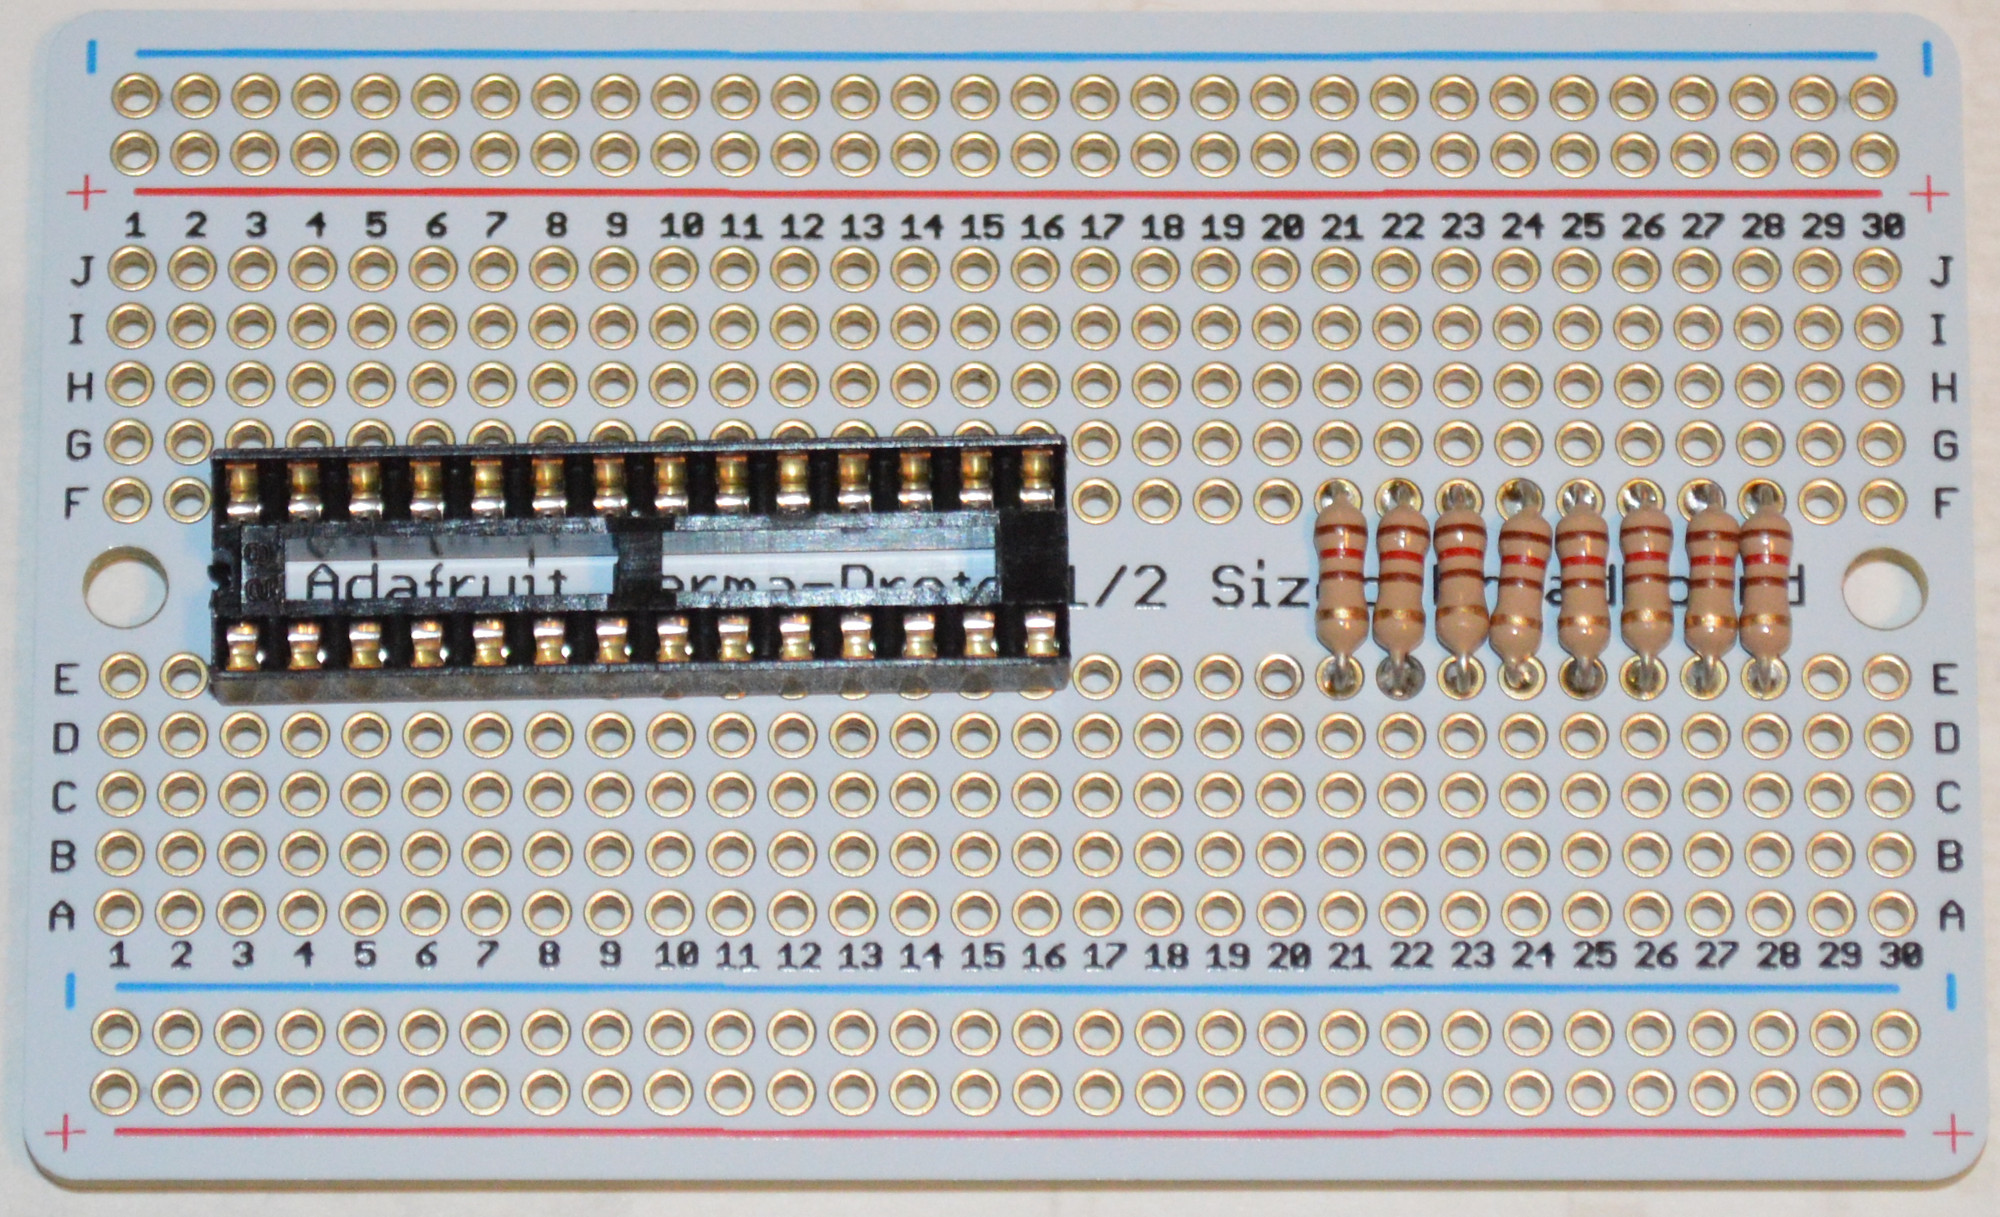
\includegraphics[width=0.9\textwidth]{../Pict/GPIO 1.jpg}
  \caption{GPIO Board with Socket and Resistors}
  \label{fig:GPIO1}
\end{figure}

\begin{figure}[ht!]
  \centering
  \includegraphics[width=0.9\textwidth]{../Pict/GPIO 2.jpg}
  \caption{GPIO Board with Socket, Resistors, and Fixed Wires}
  \label{fig:GPIO2}
\end{figure}

\begin{figure}[ht!]
  \centering
  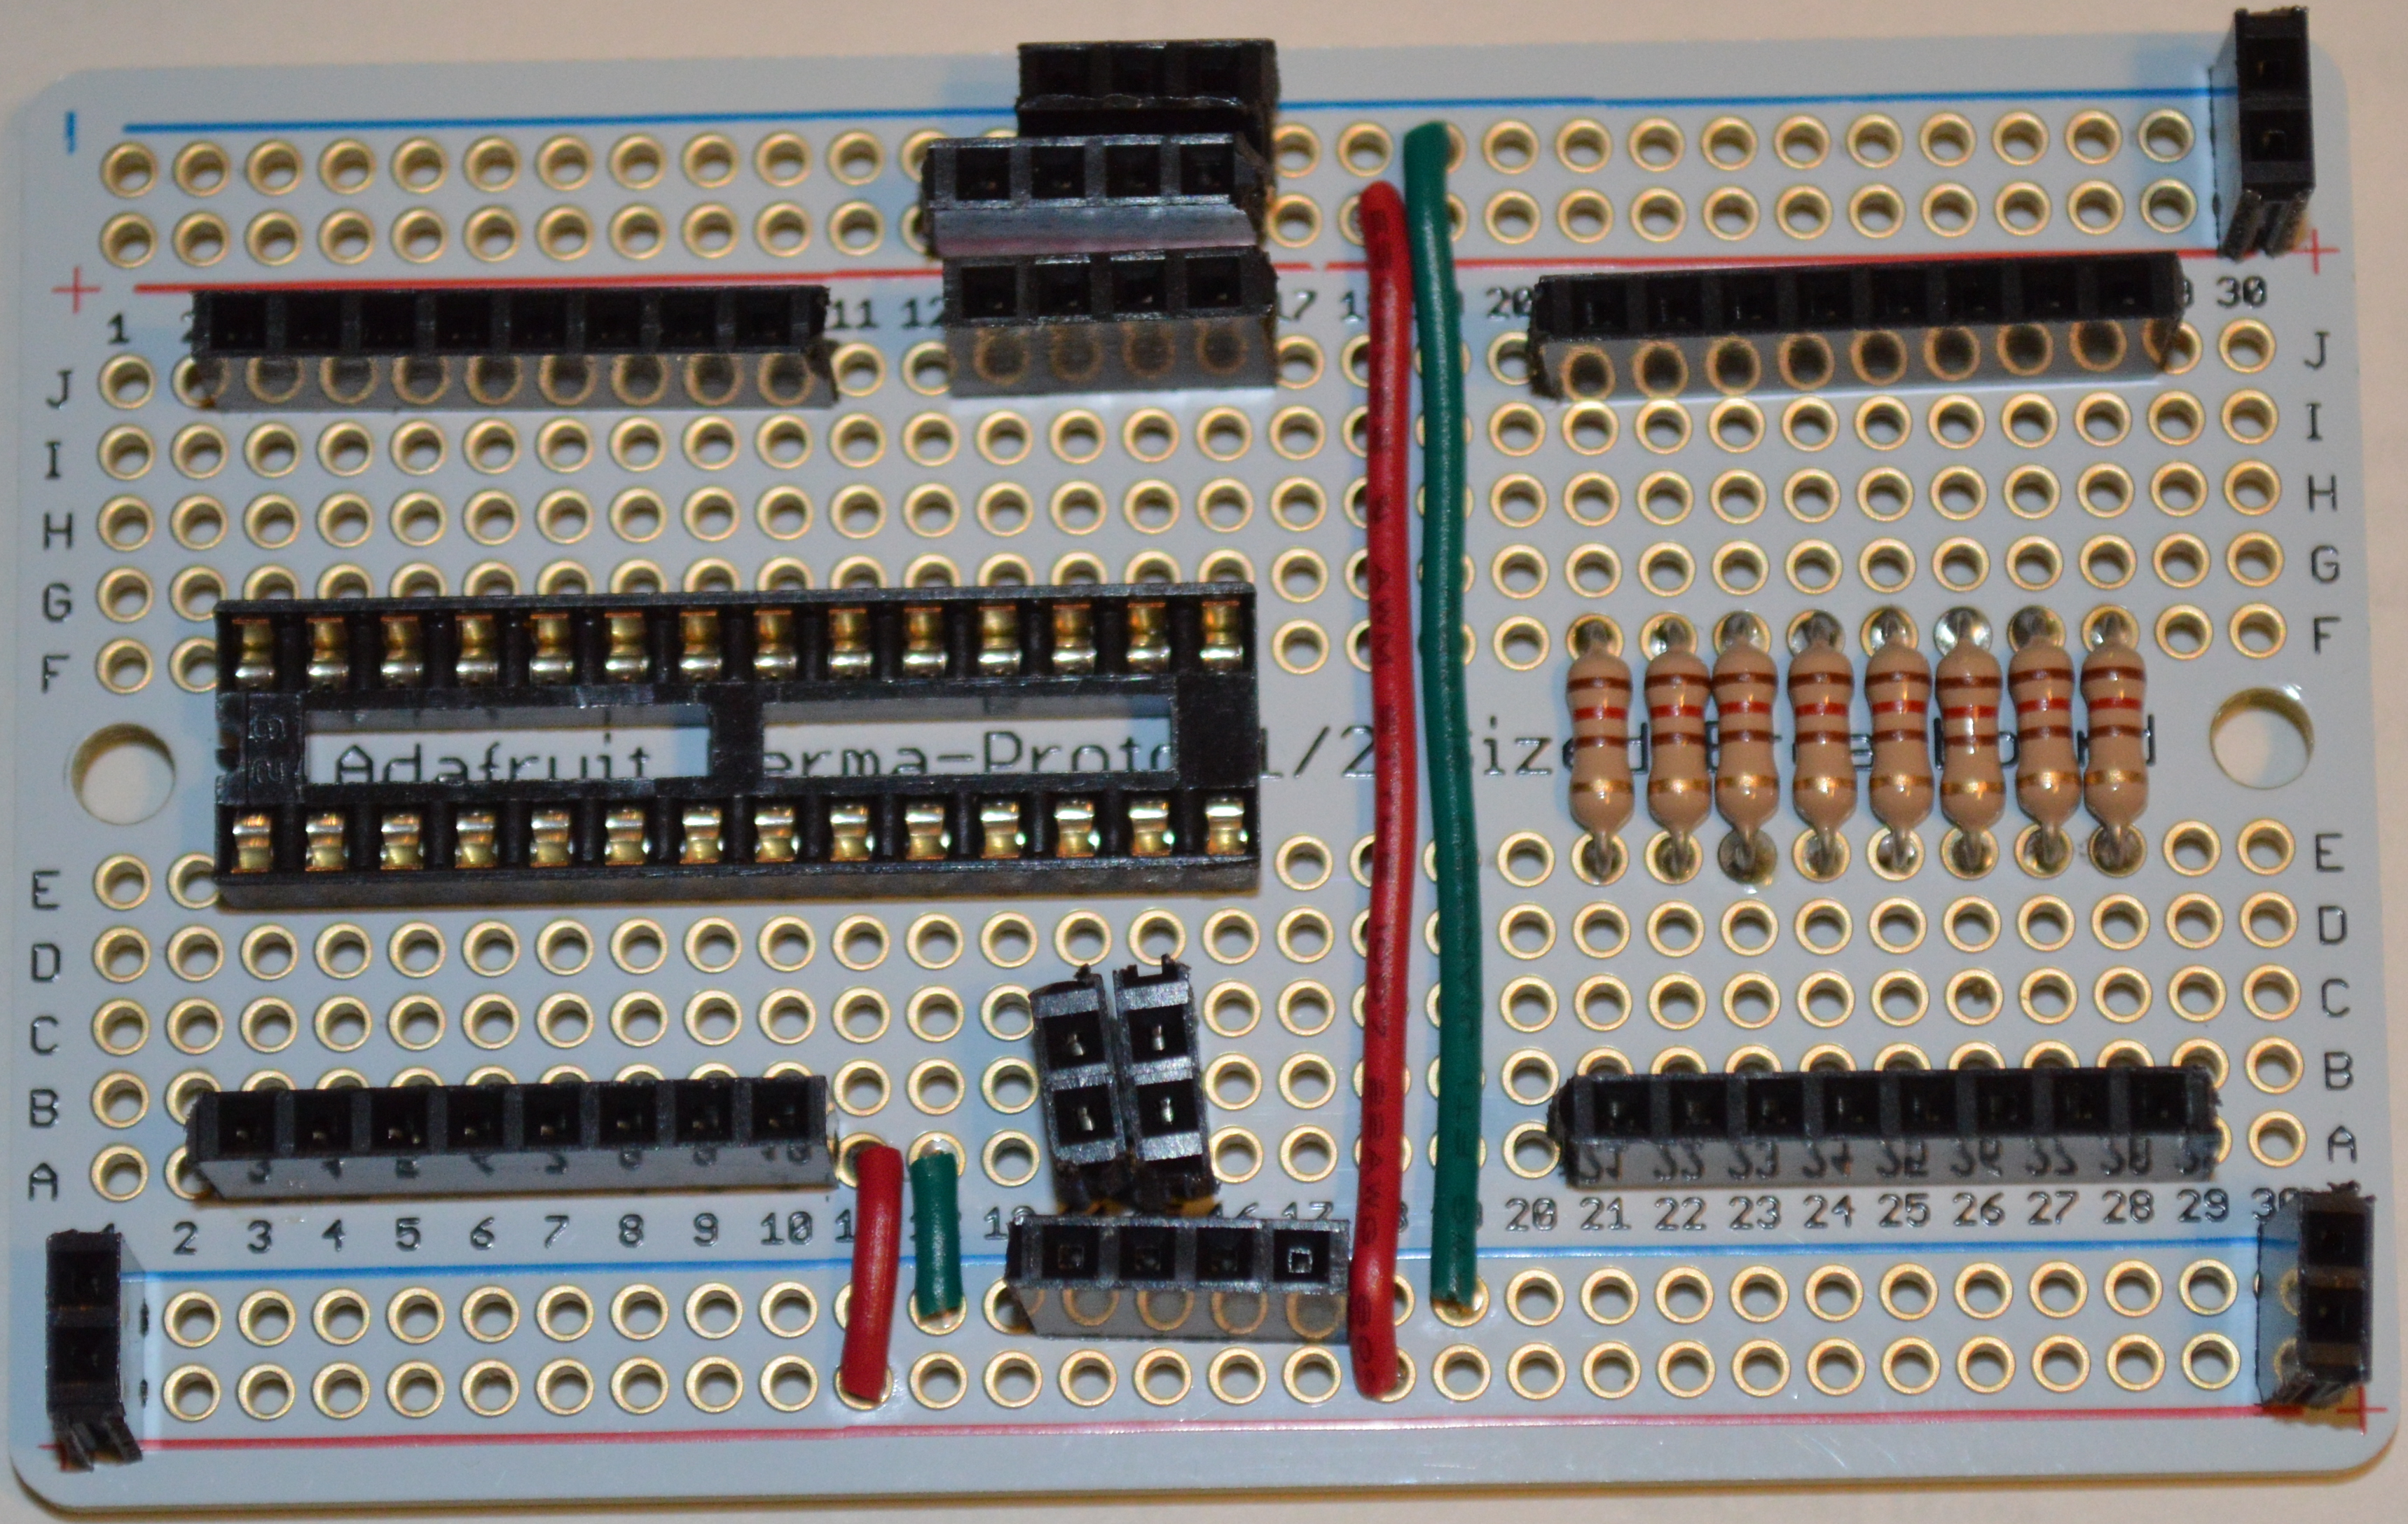
\includegraphics[width=0.9\textwidth]{../Pict/GPIO 3.jpg}
  \caption{GPIO Board with Headers}
  \label{fig:GPIO3}
\end{figure}

\clearpage
\subsection{Panel I/O Tray}
There are two discrete I/O boards on this tray.  Together they can drive up to 16 LEDs and read 16 switches.  The left board drives the LEDs and the right board reads the switches.  The connectors from left to right are: MSB LEDs, MSB switches, LSD switches, and LSB LEDs.

It turns out that 8 of the 16 GPIO pins on the MCP23017 are numbered ascending down one side of the chip and the other 8 are numbered descending down the other side.  To account for this, you can either have the jumpers cross over for two of the panel connectors (I did this in the first version), or simply rotate two of the connectors by 180\degree{}, thus putting the twist into the cable.
\begin{itemize}
  \item Attach the connectors to the tray.  See Figure \ref{fig:PanelIO1}.
  \item Attach the two Discrete I/O Boards.  See Figure \ref{fig:PanelIO2}.
  \item Add wiring for power, I2C, and board configuration (Figure \ref{fig:PanelIO3} shows the address and reset jumpers installed.  From the address jumpers, these are the control LED and control switch boards) and install the MCP23017s.  See Figure \ref{fig:PanelIO4}.  If the processor and bus cable are ready, this can be hooked up to see that the processor detects the MCP23017s.
  \item Add wiring to the connectors.  See Figures \ref{fig:PanelIO5}, \ref{fig:PanelIO6}, and \ref{fig:PanelIO7}.  Also refer to subsection \ref{subsec:PanelLED} to make sure that the connector pinouts match those of the panel being connected.
\end{itemize}

\begin{figure}[ht!]
  \centering
  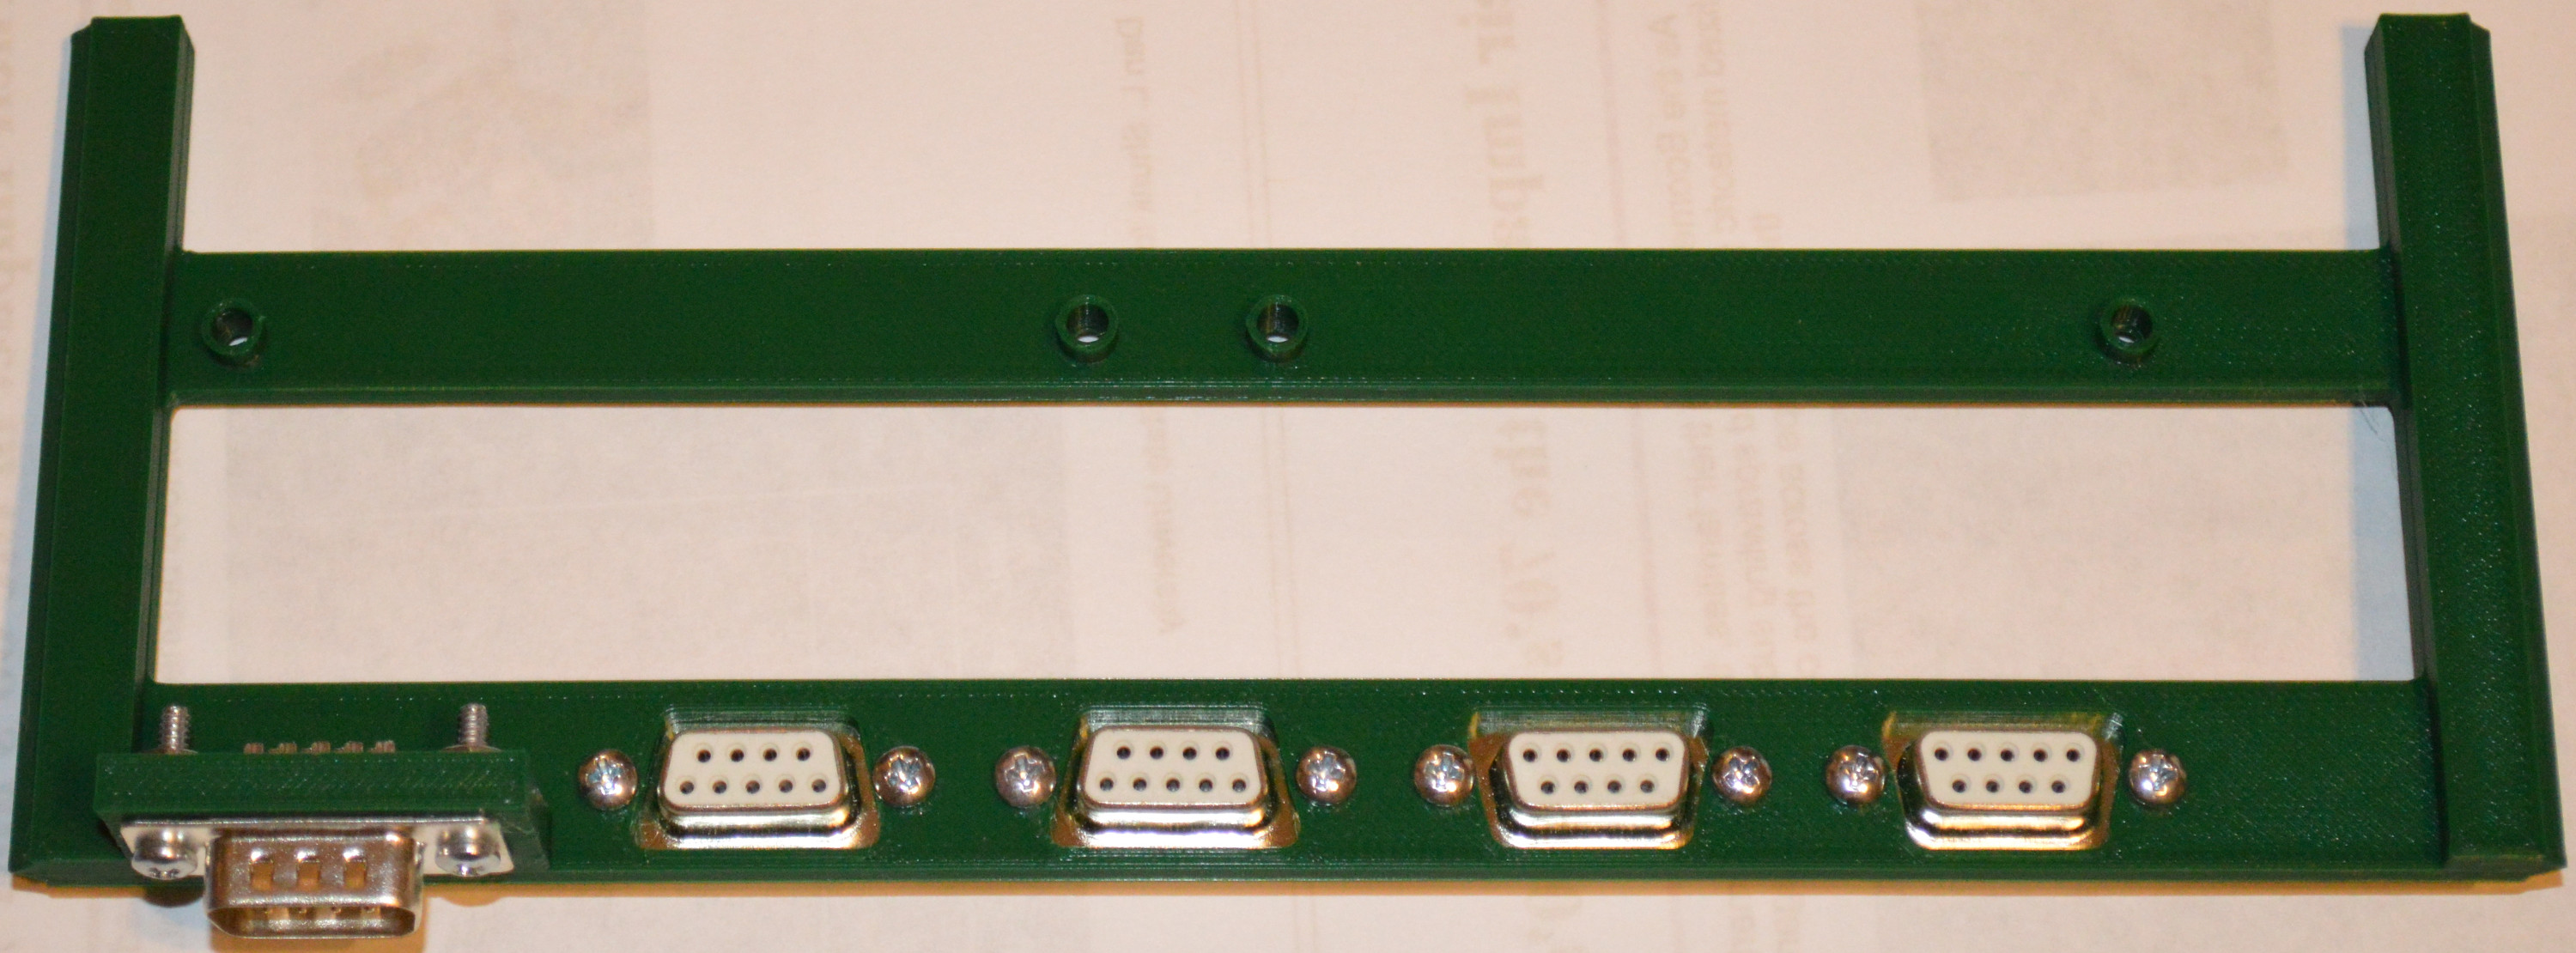
\includegraphics[width=0.9\textwidth]{../Pict/PanelIOTray1.jpg}
  \caption{Panel I/O Tray with Connectors}
  \label{fig:PanelIO1}
\end{figure}

\begin{figure}[ht!]
  \centering
  \includegraphics[width=0.9\textwidth]{../Pict/PanelIOTray2.jpg}
  \caption{Panel I/O Tray with GPIO Boards}
  \label{fig:PanelIO2}
\end{figure}

\begin{figure}[ht!]
  \centering
  \includegraphics[width=0.9\textwidth]{../Pict/PanelIOTray3.jpg}
  \caption{Panel I/O Tray with GPIO Boards with Address and Reset Jumpers Installed.  These are Control LED and Control Switch Boards}
  \label{fig:PanelIO3}
\end{figure}

\begin{figure}[ht!]
  \centering
  \includegraphics[width=0.9\textwidth]{../Pict/PanelIOTray4.jpg}
  \caption{Panel I/O Tray with GPIO Boards with Power, I2C, and MPC23017s Installed}
  \label{fig:PanelIO4}
\end{figure}

\begin{figure}[ht!]
  \centering
  \includegraphics[width=0.9\textwidth]{../Pict/PanelIOTray5.jpg}
  \caption{Panel I/O Tray with LSB LED and Switch Connectors Wired}
  \label{fig:PanelIO5}
\end{figure}

\begin{figure}[ht!]
  \centering
  \includegraphics[width=0.9\textwidth]{../Pict/PanelIOTray6.jpg}
  \caption{Panel I/O Tray with MSB LED and Switch Connectors Wired}
  \label{fig:PanelIO6}
\end{figure}

\begin{figure}[ht!]
  \centering
  \includegraphics[width=0.9\textwidth]{../Pict/PanelIOTray7.jpg}
  \caption{Back Side of Panel I/O Tray Showing Connector Wiring}
  \label{fig:PanelIO7}
\end{figure}

\clearpage
\subsection{I2C Bus Cable}
The I2C bus cable is probably the most difficult bit of soldering as you will have to add two wires to each contact in a connector.  Multiple times.  Which pairs are used for which pins isn't particularly important, but I wire pins 2 \& 6, 2 \& 7, 4 \& 8, and 5 \& 9 as pairs.  Pin 3 is left unconnected.  It is obviously important to have the same wire go to the same pin on each connector on the bus.  Figure \ref{fig:Cable1} shows an example cable.  Figure \ref{fig:Cable2} is a close-up of one of the connectors.  It is a little easier to decide ahead of time how many connectors you want on the bus.  Soldering a cable segment to an existing connector can be done, but is more difficult.

\begin{figure}[ht!]
  \centering
  \includegraphics[width=0.9\textwidth]{../Pict/Bus Cable.jpg}
  \caption{The I2C Bus Cable}
  \label{fig:Cable1}
\end{figure}

\begin{figure}[ht!]
  \centering
  \includegraphics[width=0.9\textwidth]{../Pict/Connector.jpg}
  \caption{An I2C Bus Cable Connector}
  \label{fig:Cable2}
\end{figure}

\clearpage
\subsection{Panel LEDs}
\label{subsec:PanelLED}
The wiring for the panel LEDs is similar for all panels.  The Modes Panel is shown as an example.  The LEDs on the other panels would be wired the same way.  Note the cable ties used to attach the wiring to the panel.  This also helps to keep the LEDs in place so that they don't push out.

You can choose whatever pinout you want for the connectors, however it helps if there is some reason and consistency behind it.  What I have done is to look at the connector from the back with the wide side up and assign the pins in the same order as the LEDs or switches, with the very middle pin assigned to ground (as shown in Figure \ref{fig:LED5}.  That is, the left-most pin corresponds to the left-most LED or switch, and so on.

\begin{itemize}
  \item Since CAT-5 cables are only 8 conductor, a separate ground/return wire needs to be added.  As a note of caution, I find that the orange and brown pairs are difficult to distinguish.  Be careful, otherwise you may wind up having to resolder the connector.  See Figure \ref{fig:LED5}.
  \item First using a cable tie, attach the cable to the panel.  This helps to keep the cable from moving around while the LEDs are soldered.  There is also a bare copper wire used as a ground/return wire for the LEDs.  See Figure \ref{fig:LED1}.
  \item Solder the first LED to one side of the cable.  This one is the hardest as there is only a short length of wire to work with.  See Figure \ref{fig:LED2}.
  \item Solder the next LED and add a cable tie between them.  See Figure \ref{fig:LED3}.
  \item Solder the remaining LEDs on that side and add cable ties between them.  See Figure \ref{fig:LED4}.
  \item Find a place to solder the ground/return wire from the connector to the bare LED ground/return wire.  See Figure \ref{fig:LED6}.
  \item Complete the other side of the panel.  See Figure \ref{fig:LED6}.
  \item At some point, you may wish to trim the leads on the LEDs.
\end{itemize}

\begin{figure}[ht!]
  \centering
  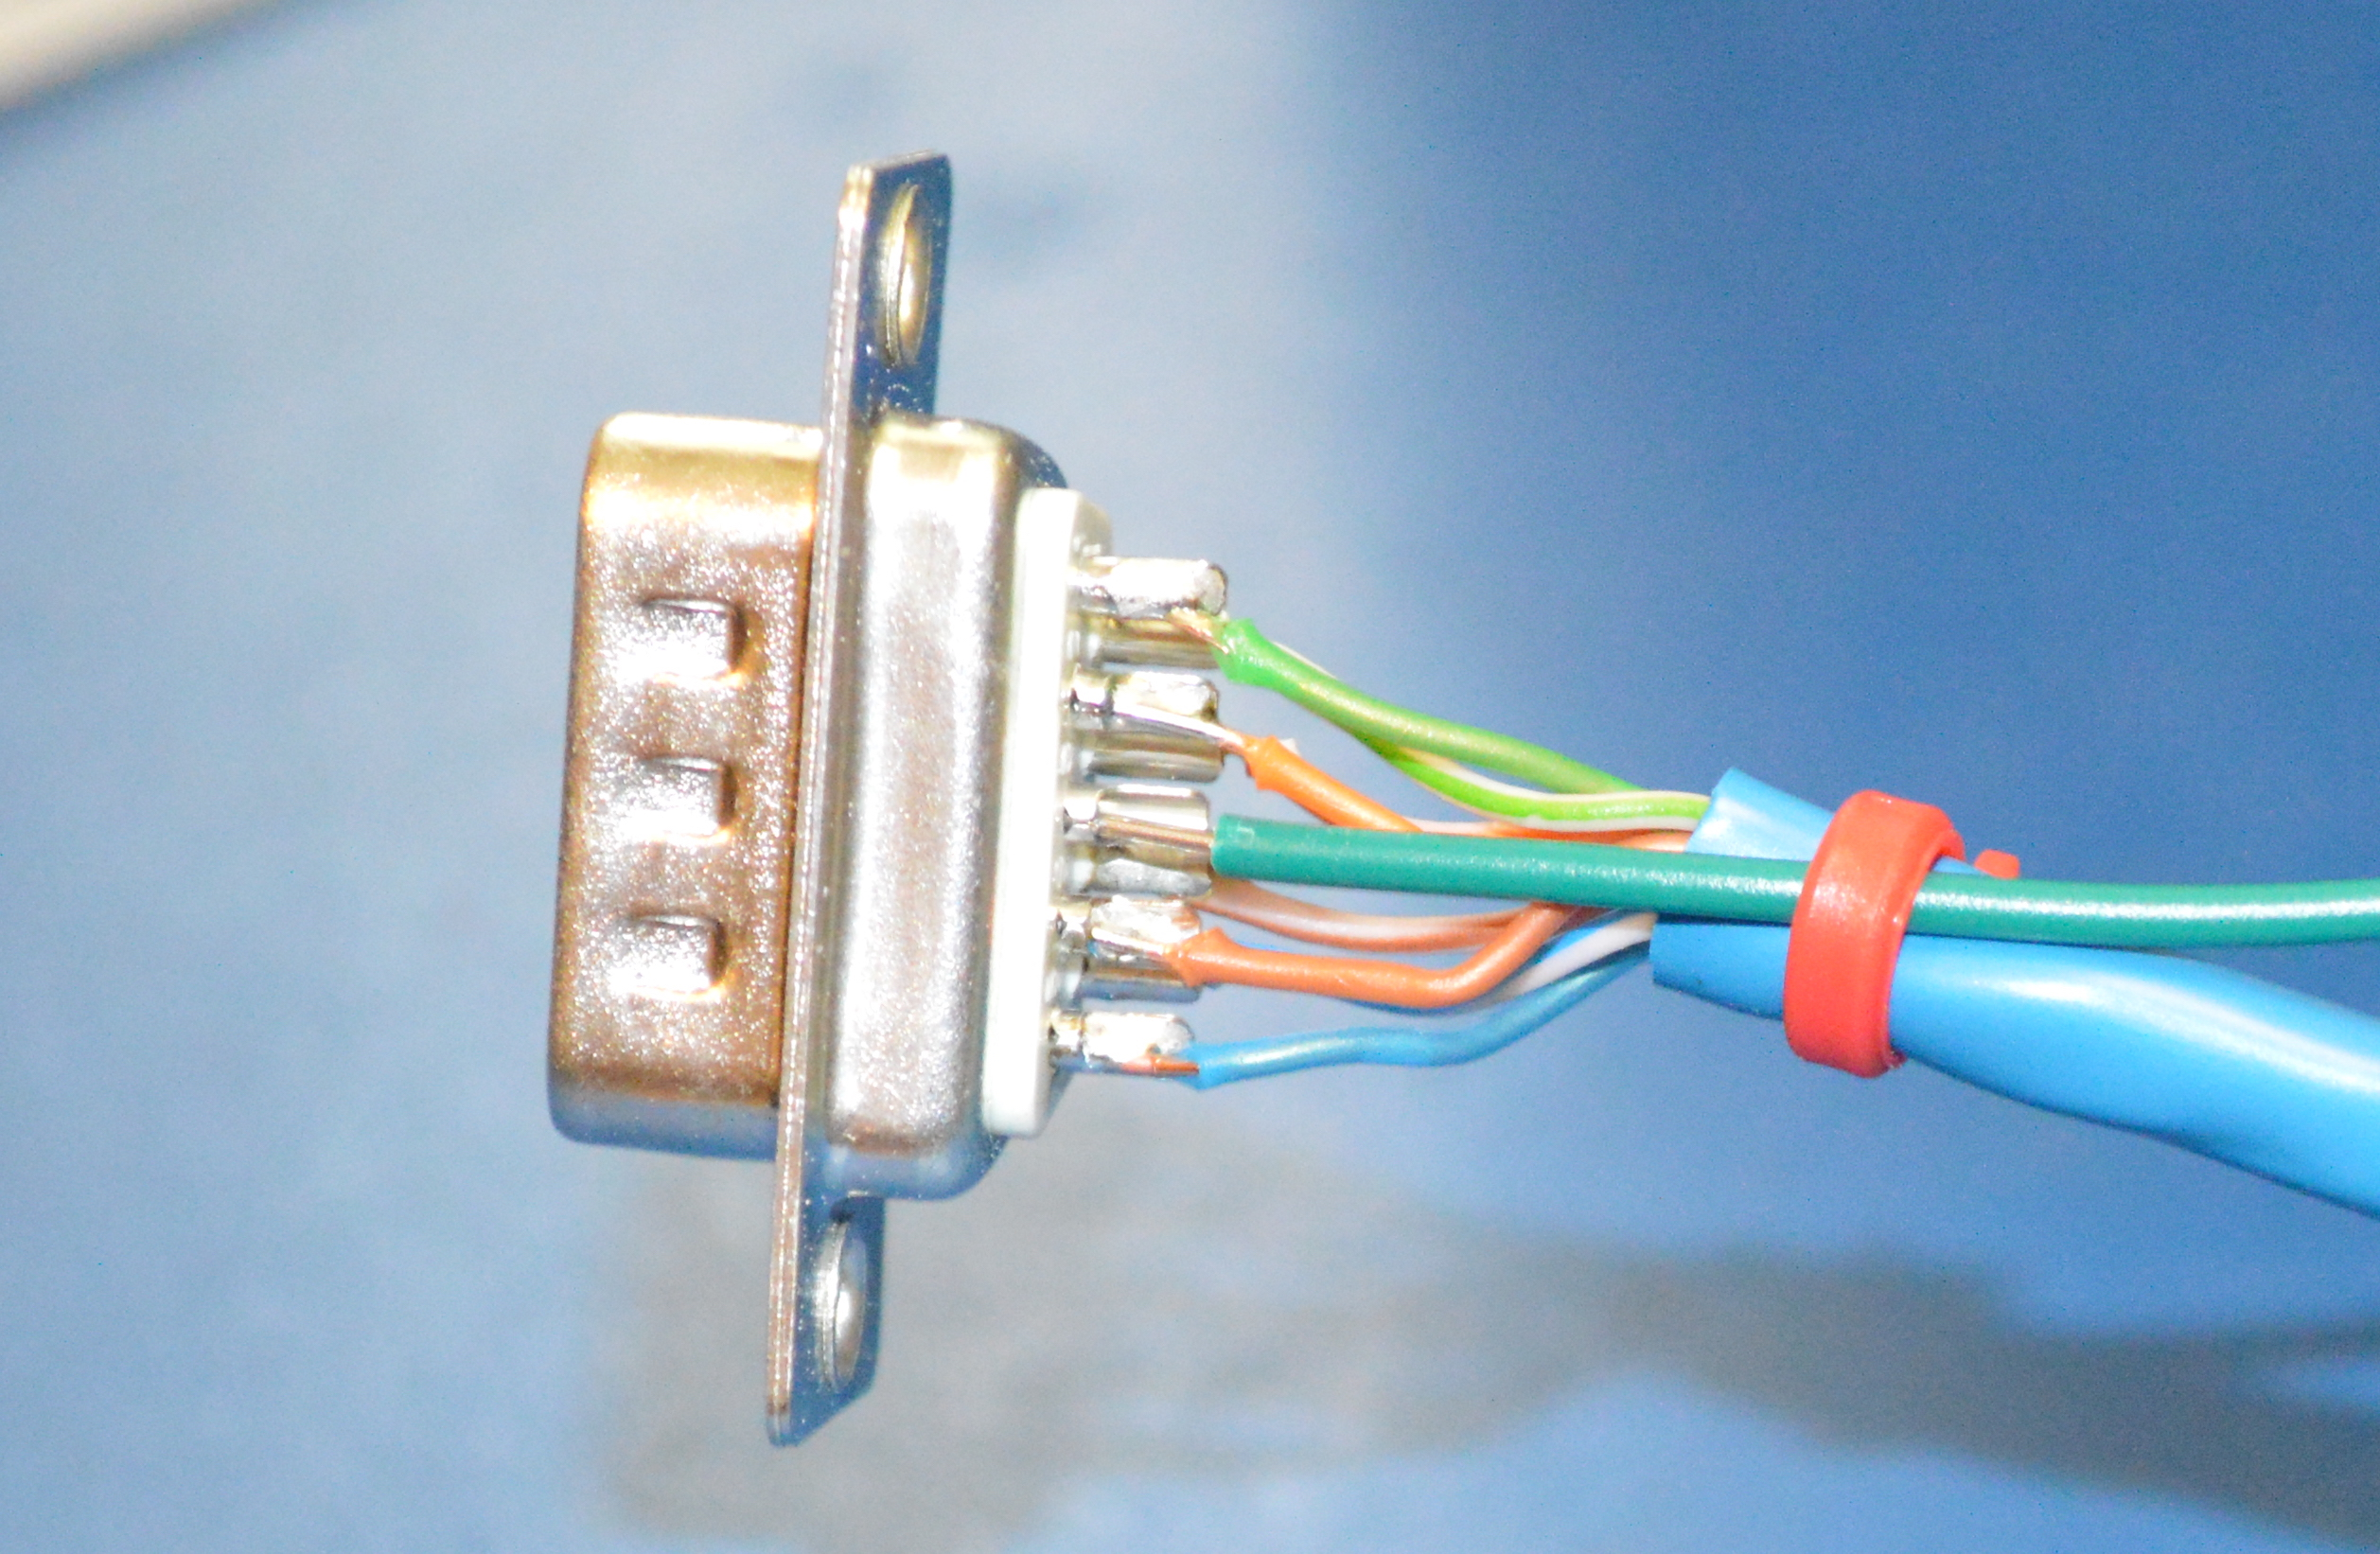
\includegraphics[width=0.9\textwidth]{../Pict/LEDs5.jpg}
  \caption{LED Panel Connector with Ground Wire}
  \label{fig:LED5}
\end{figure}

\begin{figure}[ht!]
  \centering
  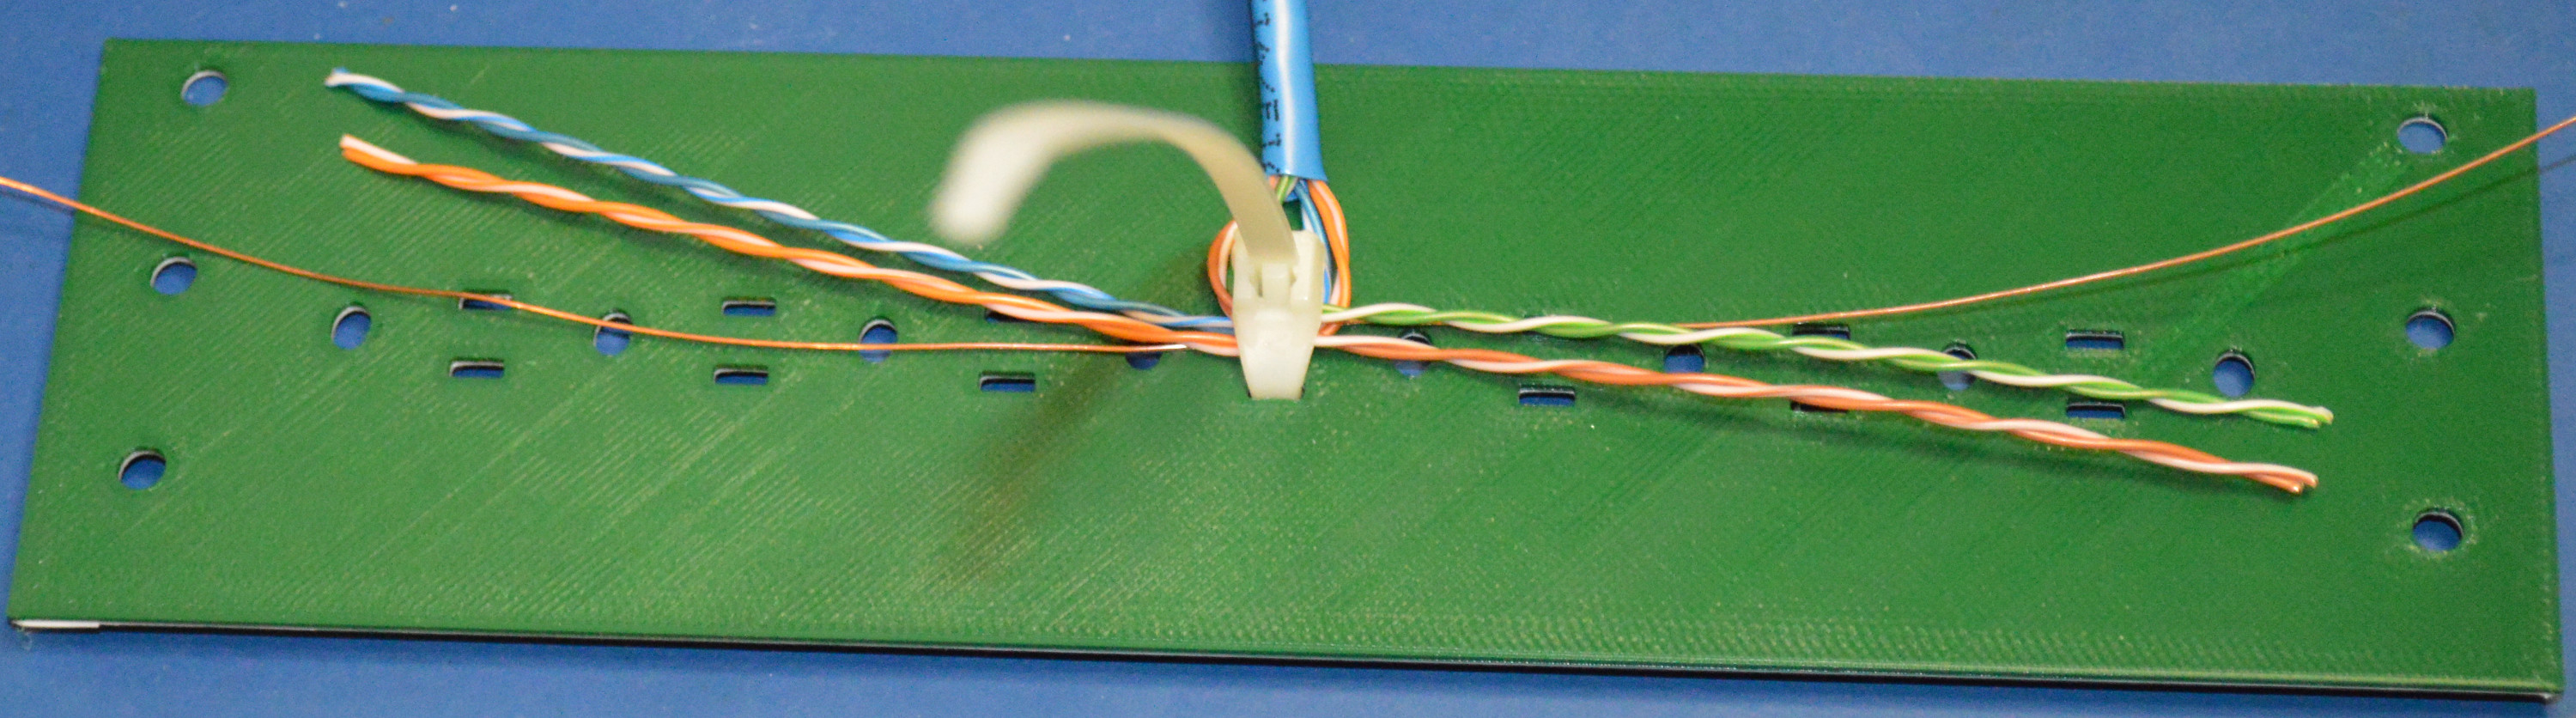
\includegraphics[width=0.9\textwidth]{../Pict/LEDs1.jpg}
  \caption{Attach the Cable to the Panel}
  \label{fig:LED1}
\end{figure}

\begin{figure}[ht!]
  \centering
  \includegraphics[width=0.9\textwidth]{../Pict/LEDs2.jpg}
  \caption{Solder the First LED}
  \label{fig:LED2}
\end{figure}

\begin{figure}[ht!]
  \centering
  \includegraphics[width=0.9\textwidth]{../Pict/LEDs3.jpg}
  \caption{Solder the Second LED and Add a Cable Tie}
  \label{fig:LED3}
\end{figure}

\begin{figure}[ht!]
  \centering
  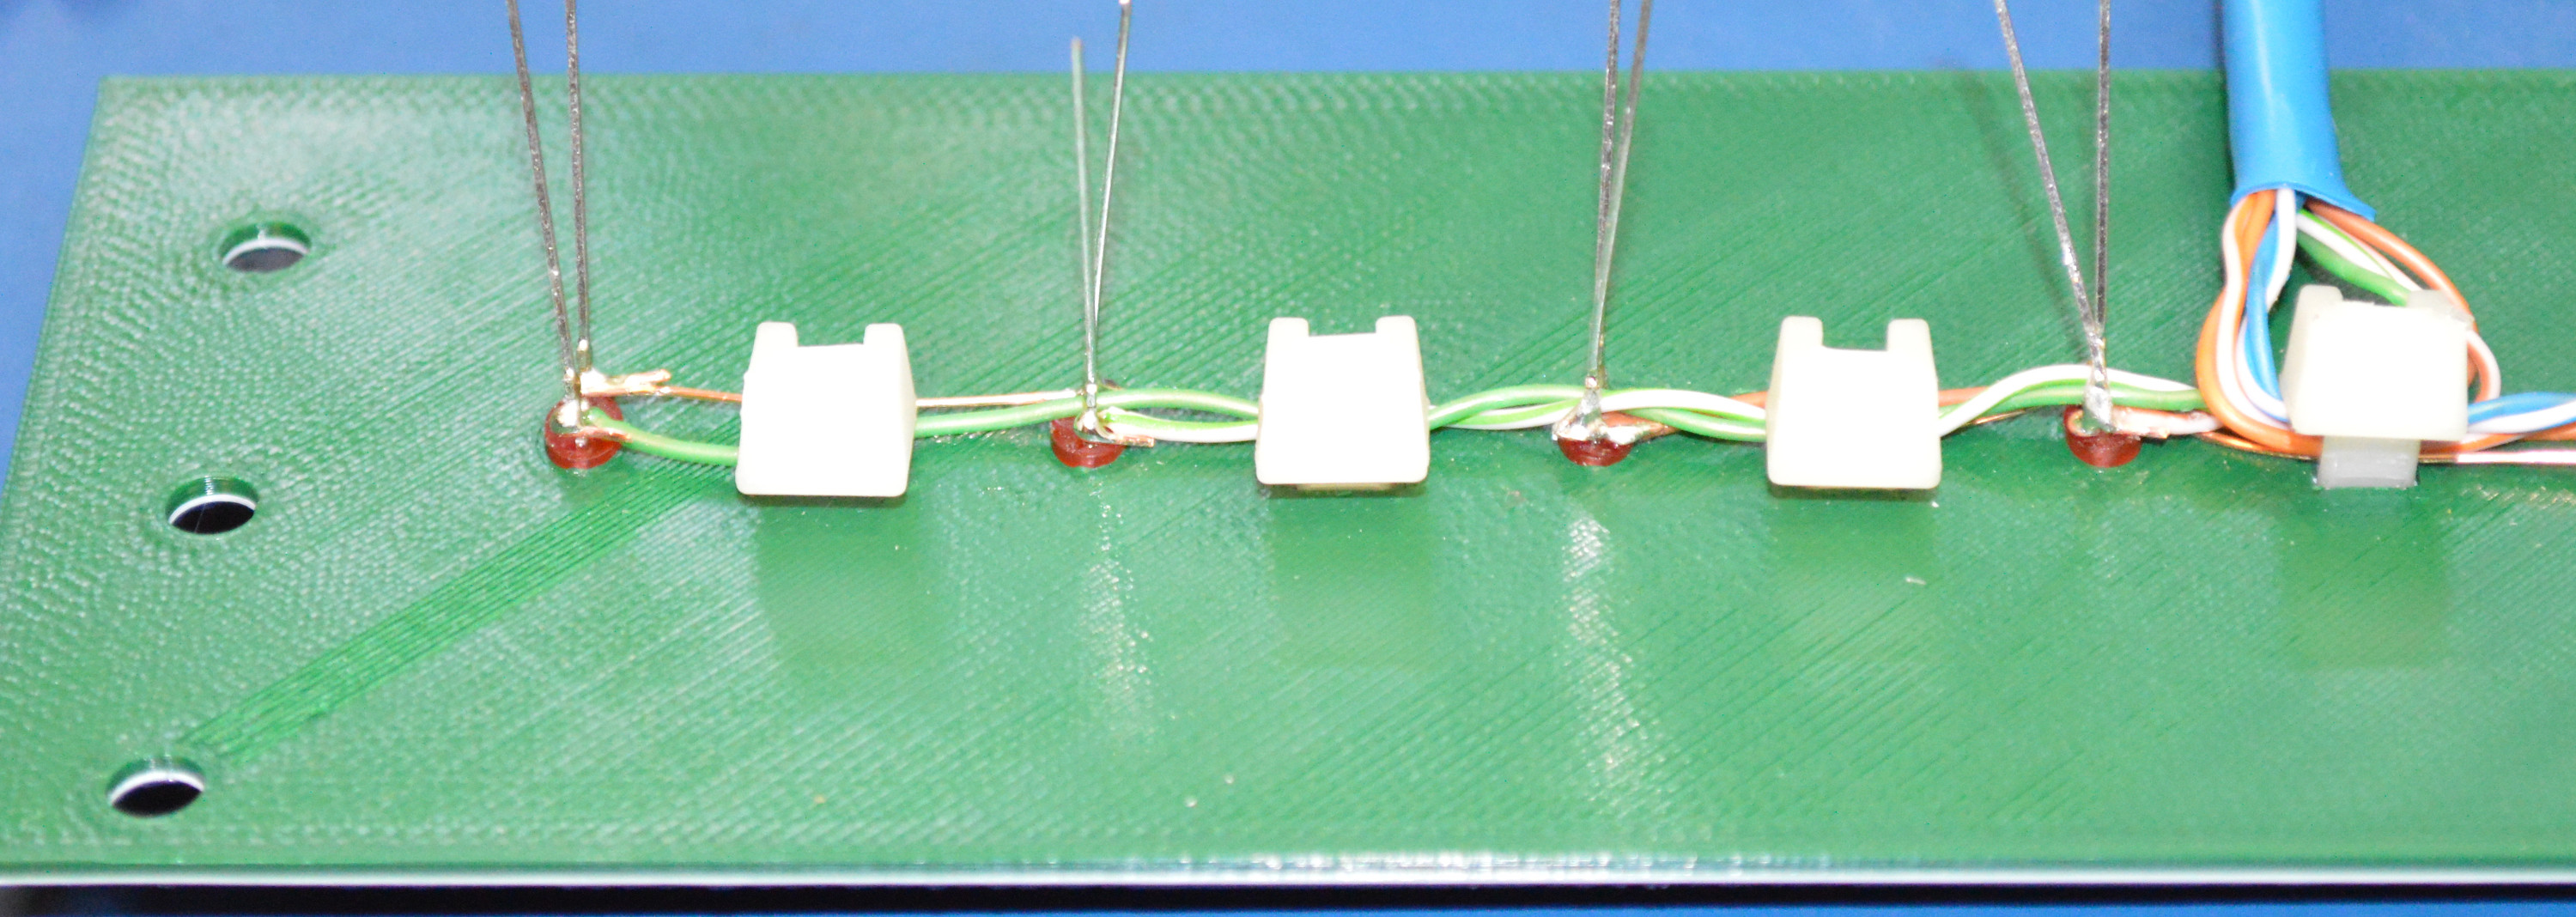
\includegraphics[width=0.9\textwidth]{../Pict/LEDs4.jpg}
  \caption{Solder the Remaining LEDs on That Side and Add Cable Ties}
  \label{fig:LED4}
\end{figure}

\begin{figure}[ht!]
  \centering
  \includegraphics[width=0.9\textwidth]{../Pict/LEDs6.jpg}
  \caption{The Completed Panel}
  \label{fig:LED6}
\end{figure}

\clearpage
\subsection{Panel Switches}
My implementation uses SPST switches where the center connector is common.  When the switch is in the up position, the center and lower connector are connected.  When the switch is in the down position, the center and upper connector are connected.  The MCP23017s have an optional pullup for each input, thus the switches can be used in an open-ground configuration.  The top connectors are tied together and connected to ground.  The center connectors are connected to the individual input pins.
\begin{itemize}
  \item Install the switches as shown in Figure \ref{fig:Switch1}.  This example shows a control panel that only has six switches.
  \item Install the wiring for the switches as shown in Figure \ref{fig:Switch2}.  Since the control panel has only six switches, one of the cable pairs is unused.
  \item Finally, install the LEDs in the panel as described in Section \ref{subsec:PanelLED} and shown in Figure \ref{fig:Switch3}.
\end{itemize}
\begin{figure}[ht!]
  \centering
  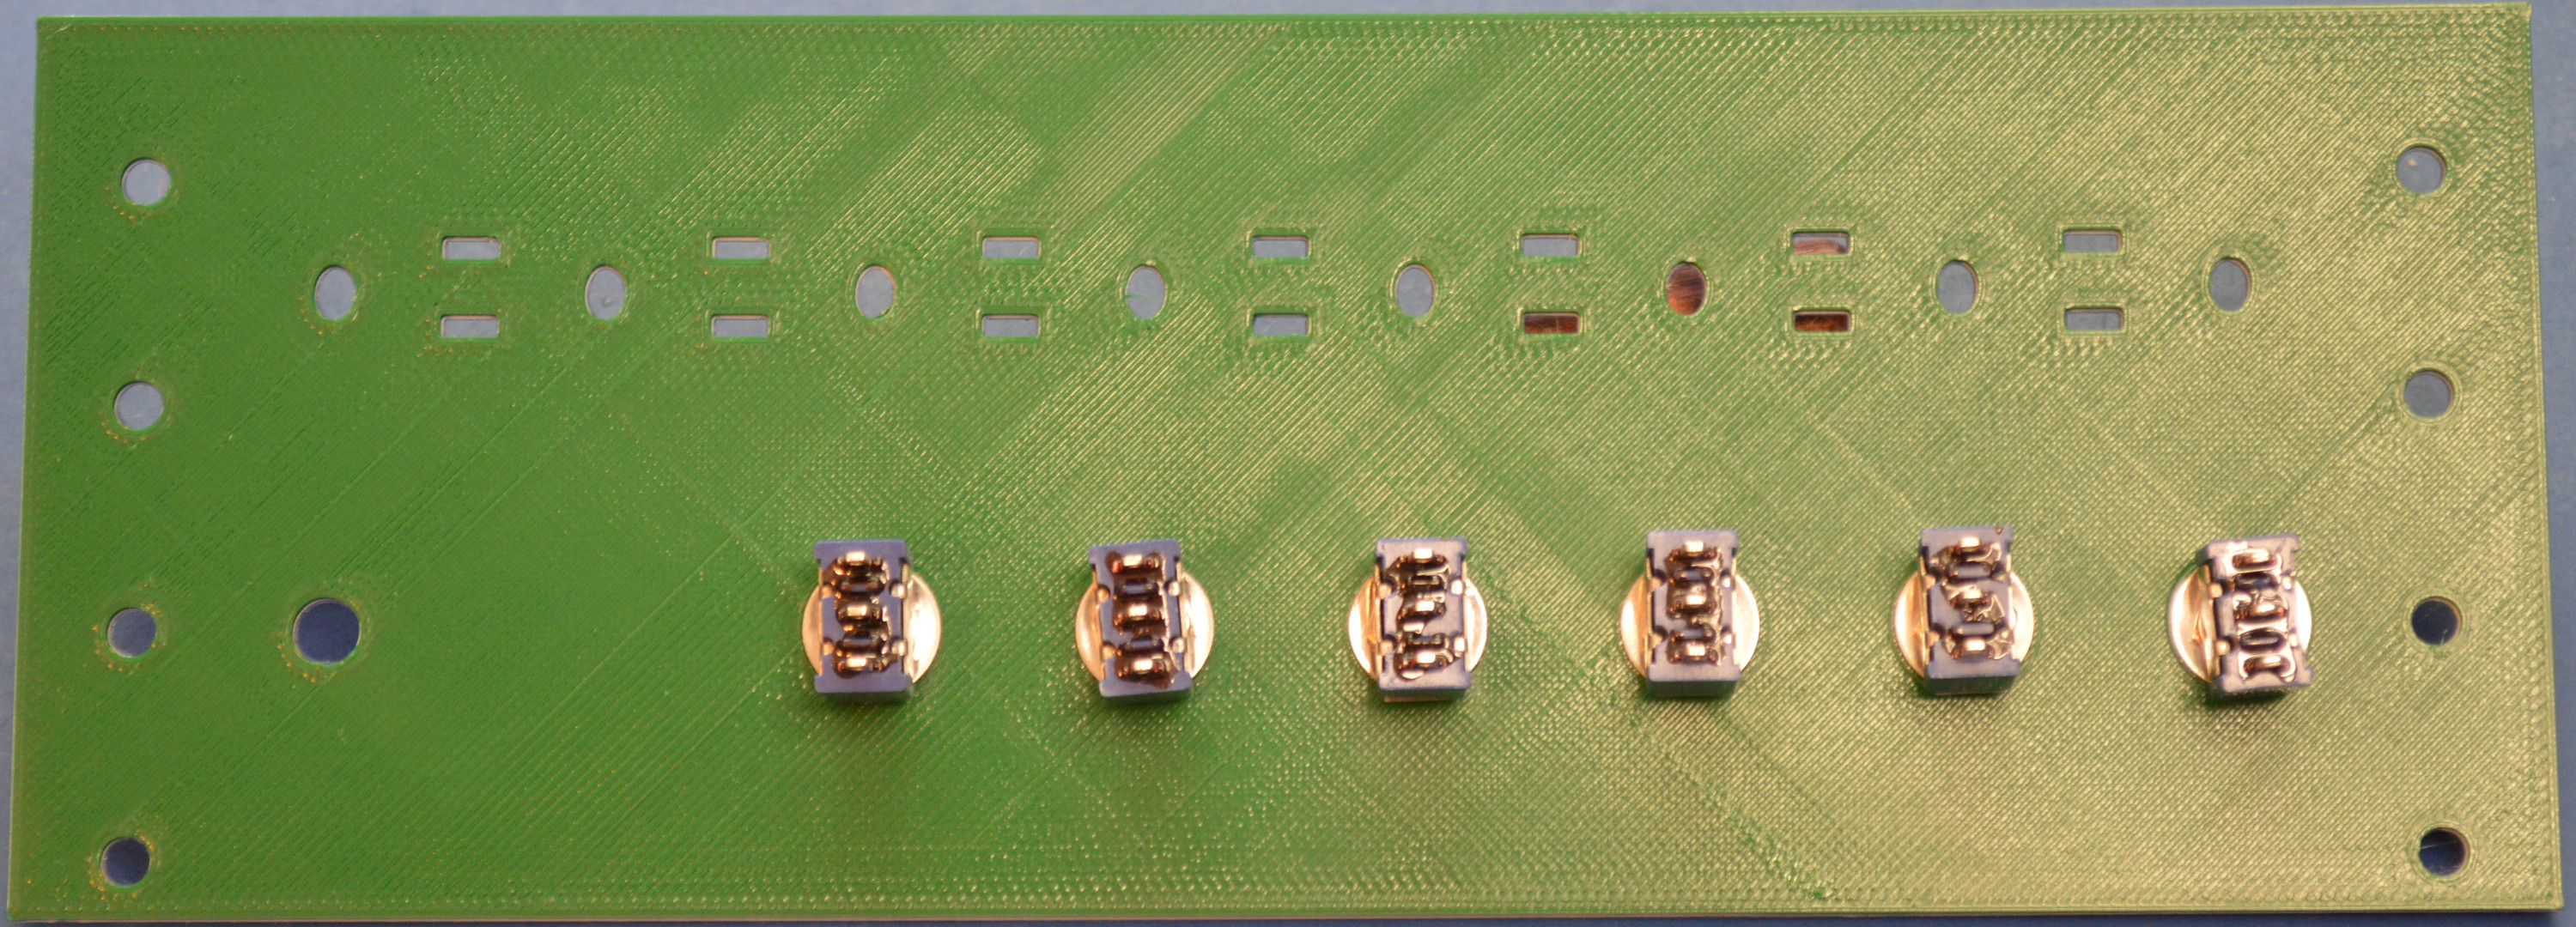
\includegraphics[width=0.9\textwidth]{../Pict/Switch1.jpg}
  \caption{Control Panel Switches Showing Switches Installed}
  \label{fig:Switch1}
\end{figure}

\begin{figure}[ht!]
  \centering
  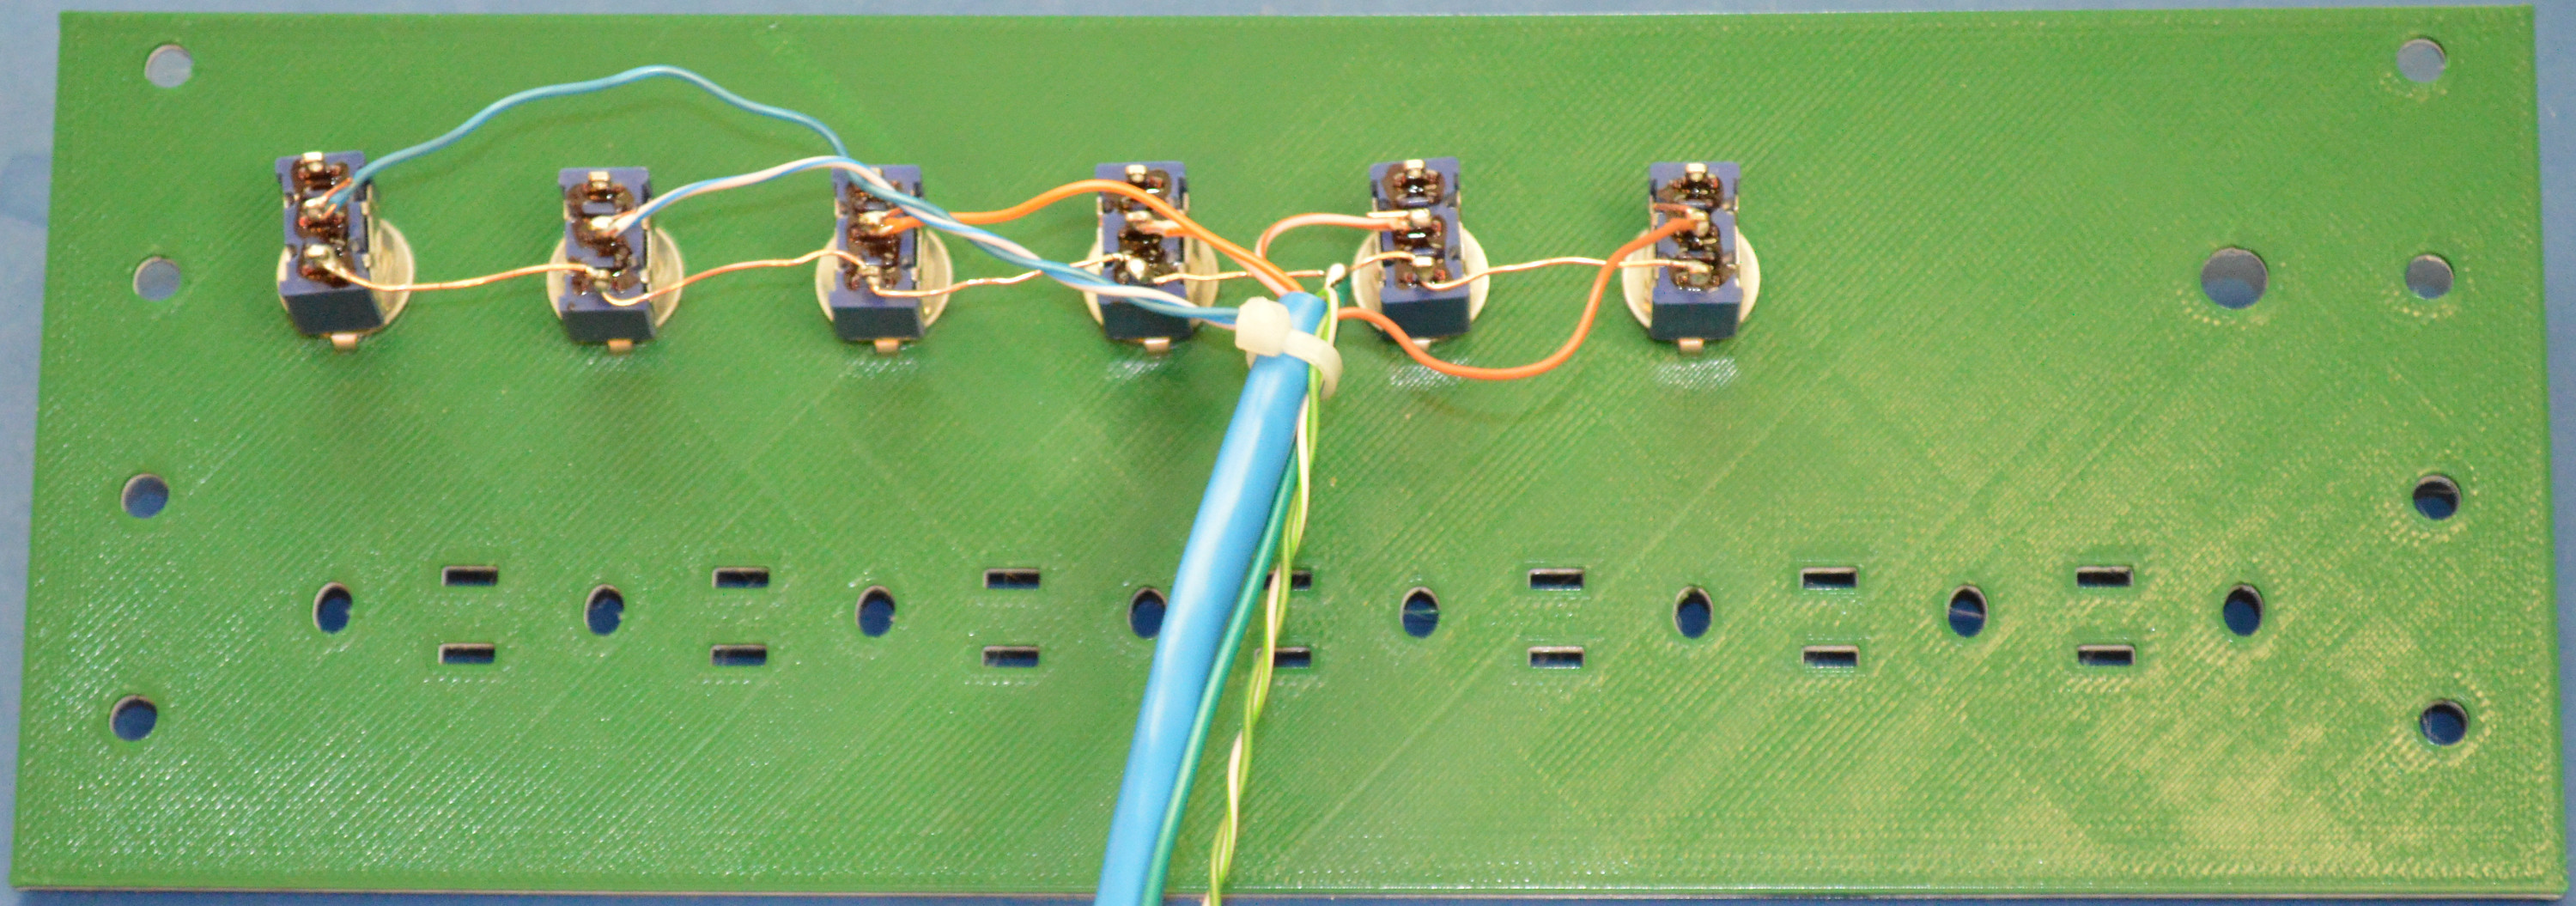
\includegraphics[width=0.9\textwidth]{../Pict/Switch2.jpg}
  \caption{Control Panel Switches Showing Wiring}
  \label{fig:Switch2}
\end{figure}

\begin{figure}[ht!]
  \centering
  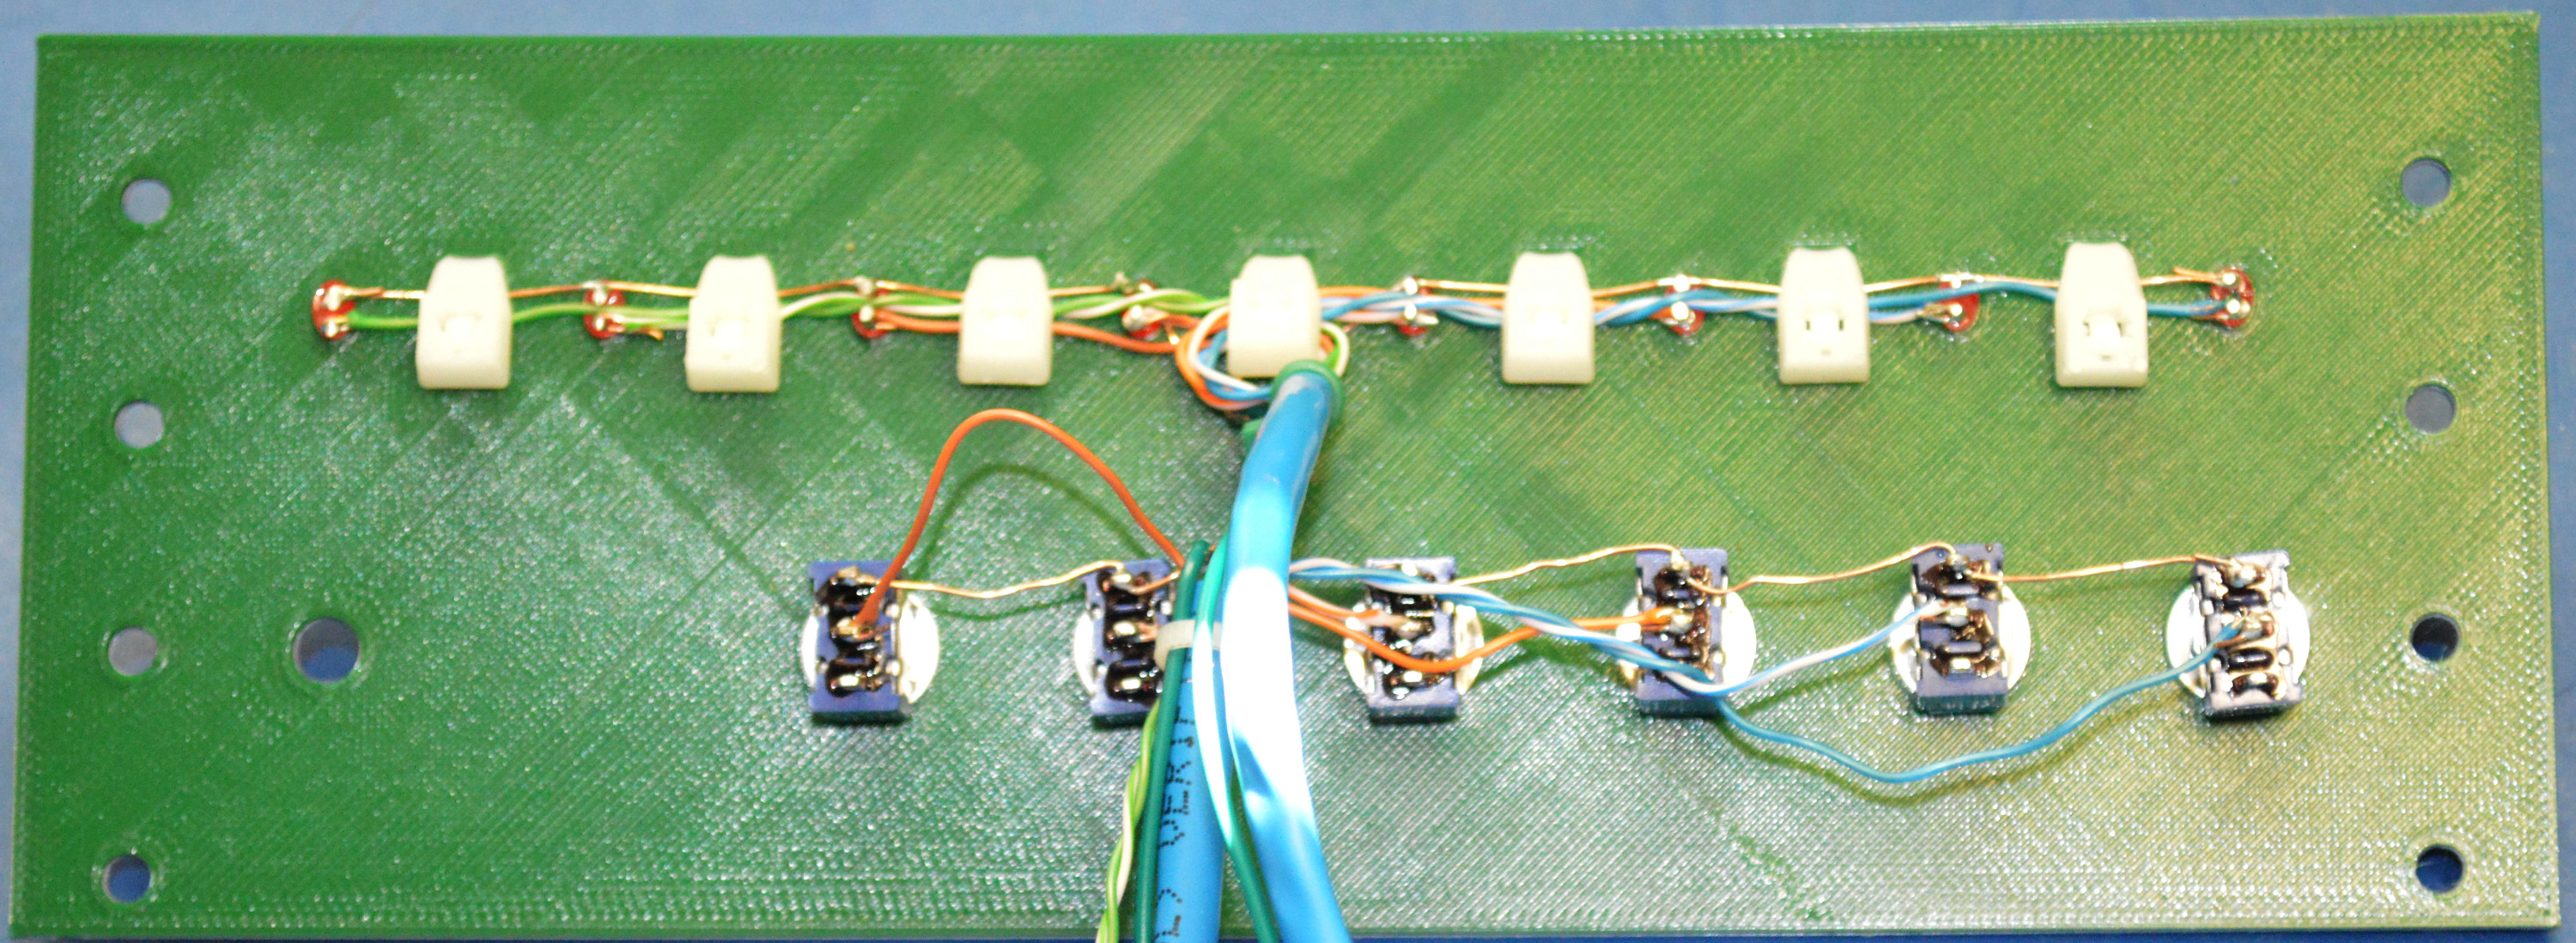
\includegraphics[width=0.9\textwidth]{../Pict/Switch3.jpg}
  \caption{Control Panel with Switches and LEDs Installed and Wired}
  \label{fig:Switch3}
\end{figure}

\section{Power}
You can go with just plugging a USB power adapter into the micro-USB connector on the Raspberry PI, or you can get fancier.  There is a model for a power panel that has cutouts for micro-USB and a USB-B panel mount connectors.  Adafruit offers a number of panel mount USB to various USB adapters.  You can just use one of these.  If you want to get fancier, you can cut open the USB cable and insert the power switch in series with the power conductor.  At this point, you are on your own.  Be careful!

%----------------------------------------------------------
\chapter{Software}
\section{Overview}
Currently, the software has two main interfaces.  The first is the switches and lights.  The second is a web interface.

\section{Simulation}

\begin{table}
  \label{tbl:Simulations}
  \caption{Simulations Available}
  \centering
  \begin{tabular}{|r|l|}
    \hline
    0 & Copy Switch Values\\
    1 & Count\\
    2 & 16-bit Scan\\
    3 & 16-bit Bounce\\
    4 & Fibonacci Sequence\\
    9 & Count\\
    10 & 32-bit Scan\\
    11 & 32-bit Bounce\\
    12 & Fibonacci Sequence\\
    \hline
    other & Copy Switch Values\\
    \hline
  \end{tabular}
\end{table}

There are a number of ``simulations'' available for testing or display.  The desired simulation can be selected either using the switches, or, if enabled, using the web interface.  The following is a description of the control switches:
\begin{itemize}
  \item The \switch{Power}{Off} switch is intended to be hardwired to the power supply.  There is no program function.
  \item The \position{Exam} switch has no current function.
  \item The \position{Dep} switch is used to select which simulation to run.
  \item The \switch{Addr}{Data} switch has no current function.
  \item The \switch{Auto}{Man} switch enables simulation selection by the web interface when in the \position{Auto} position.
  \item The \switch{Start}{Stop} switch sets all simulation variables to their initial state when moved to the \position{Start} position.  It also must be in the \position{Start} position for the simulation to run.
  \item The \switch{Run}{Pause} switch temporarily pauses a simulation when in the \position{Pause} position.  The simulation continues running without initialization when the switch is moved to the \position{Run} position.
\end{itemize}

Note that for a simulation to run, both the \switch{Start}{Stop} switch must be in the \position{Start} position and the \switch{Run}{Pause} switch must be in the \position{Run} position.

On program initialization, simulation 0 (Copy Switch Values) is selected by default.  To select a different simulation, make sure that either the \switch{Run}{Pause} switch is in the \position{Pause} position or the \switch{Start}{Stop} switch is in the \position{Stop} position.  Then:
\begin{itemize}
  \item Using the \switch{Addr}{Data} switches, select the desired simulation as listed in Table \ref{tbl:Simulations}.
  \item Move the \position{Dep} switch to the \position{Dep} position.  You may need to move it to the unlabeled position first.
  \item Move the \position{Dep} switch to the unlabeled position.
  \item Move the \switch{Run}{Pause} switch to the \position{Run} position.
  \item Move the \switch{Start}{Stop} switch to the \position{Start} position.
\end{itemize}

Unless you wish to reset the simulation values, you should always leave the \switch{Start}{Stop} switch in the \position{Start} position.

\section{Web Server}
The web interface is available on port 31415 (configurable in web.adb).  It uses plain, unencrypted HTTP.

\section{Other Software}
To enhance the experience, you can install some old computer emulation software (such as simh, available at https://github.com/simh/simh).  Note that this will run completely independent from the lights and switch in this project.

\end{document}

